%%%%%%%% ICML 2025 EXAMPLE LATEX SUBMISSION FILE %%%%%%%%%%%%%%%%%

\documentclass{article}

% Recommended, but optional, packages for figures and better typesetting:
\usepackage{microtype}
\usepackage{graphicx}
\usepackage{subcaption}
\usepackage{booktabs} % for professional tables
% hyperref makes hyperlinks in the resulting PDF.
% If your build breaks (sometimes temporarily if a hyperlink spans a page)
% please comment out the following usepackage line and replace
% \usepackage{icml2025} with \usepackage[nohyperref]{icml2025} above.
\usepackage{hyperref}



% Attempt to make hyperref and algorithmic work together better:
\newcommand{\theHalgorithm}{\arabic{algorithm}}

% Use the following line for the initial blind version submitted for review:
\usepackage{icml2025}

% If accepted, instead use the following line for the camera-ready submission:
%\usepackage[accepted]{icml2025}

% For theorems and such
\usepackage{amsmath}
\usepackage{amssymb}
\usepackage{mathtools}
\usepackage{amsthm}

% if you use cleveref..
\usepackage[capitalize,noabbrev]{cleveref}

%%%%%%%%%%%%%%%%%%%%%%%%%%%%%%%%
% THEOREMS
%%%%%%%%%%%%%%%%%%%%%%%%%%%%%%%%
\theoremstyle{plain}
\newtheorem{theorem}{Theorem}[section]
\newtheorem{proposition}[theorem]{Proposition}
\newtheorem{lemma}[theorem]{Lemma}
\newtheorem{corollary}[theorem]{Corollary}
\theoremstyle{definition}
\newtheorem{definition}[theorem]{Definition}
\newtheorem{assumption}[theorem]{Assumption}
\theoremstyle{remark}
\newtheorem{remark}[theorem]{Remark}

% Todonotes is useful during development; simply uncomment the next line
%    and comment out the line below the next line to turn off comments
%\usepackage[disable,textsize=tiny]{todonotes}
\usepackage[textsize=tiny]{todonotes}


% The \icmltitle you define below is probably too long as a header.
% Therefore, a short form for the running title is supplied here:
\icmltitlerunning{Submission and Formatting Instructions for ICML 2025}

\begin{document}

\twocolumn[
\icmltitle{Dataset Distillation by Learning Exclusive Information}

% It is OKAY to include author information, even for blind
% submissions: the style file will automatically remove it for you
% unless you've provided the [accepted] option to the icml2025
% package.

% List of affiliations: The first argument should be a (short)
% identifier you will use later to specify author affiliations
% Academic affiliations should list Department, University, City, Region, Country
% Industry affiliations should list Company, City, Region, Country

% You can specify symbols, otherwise they are numbered in order.
% Ideally, you should not use this facility. Affiliations will be numbered
% in order of appearance and this is the preferred way.
\icmlsetsymbol{equal}{*}

\begin{icmlauthorlist}
\icmlauthor{Firstname1 Lastname1}{equal,yyy}
\icmlauthor{Firstname2 Lastname2}{equal,yyy,comp}
\icmlauthor{Firstname3 Lastname3}{comp}
\icmlauthor{Firstname4 Lastname4}{sch}
\icmlauthor{Firstname5 Lastname5}{yyy}
\icmlauthor{Firstname6 Lastname6}{sch,yyy,comp}
\icmlauthor{Firstname7 Lastname7}{comp}
%\icmlauthor{}{sch}
\icmlauthor{Firstname8 Lastname8}{sch}
\icmlauthor{Firstname8 Lastname8}{yyy,comp}
%\icmlauthor{}{sch}
%\icmlauthor{}{sch}
\end{icmlauthorlist}

\icmlaffiliation{yyy}{Department of XXX, University of YYY, Location, Country}
\icmlaffiliation{comp}{Company Name, Location, Country}
\icmlaffiliation{sch}{School of ZZZ, Institute of WWW, Location, Country}

\icmlcorrespondingauthor{Firstname1 Lastname1}{first1.last1@xxx.edu}
\icmlcorrespondingauthor{Firstname2 Lastname2}{first2.last2@www.uk}

% You may provide any keywords that you
% find helpful for describing your paper; these are used to populate
% the "keywords" metadata in the PDF but will not be shown in the document
\icmlkeywords{Machine Learning, ICML}

\vskip 0.3in
]

% this must go after the closing bracket ] following \twocolumn[ ...

% This command actually creates the footnote in the first column
% listing the affiliations and the copyright notice.
% The command takes one argument, which is text to display at the start of the footnote.
% The \icmlEqualContribution command is standard text for equal contribution.
% Remove it (just {}) if you do not need this facility.

%\printAffiliationsAndNotice{}  % leave blank if no need to mention equal contribution
\printAffiliationsAndNotice{\icmlEqualContribution} % otherwise use the standard text.

\begin{abstract}
Dataset distillation has emerged as a prominent area of research, aiming to compress large, original datasets into compact, lightweight synthetic datasets. Although existing works have shown their effectiveness on small scale datasets, they struggle to maintain performance on large scale datasets. Our analysis reveals that conventional dataset distillation methods have a bias towards generating synthetic images that mainly capture the easy samples of the real dataset. Although this bias is actually beneficial for small scale datasets, larger datasets require synthetic images to be diverse, capturing not only the easy samples, but also the hard samples of the real dataset. To this end, we propose a novel dataset distillation framework that generates synthetic images in multiple small segments, where each segment is distilled by matching a small portion of the whole dataset. Each portion is obtained by filtering out images prior to distillation, and each synthetic segment is distilled using a different set of images . This method facilitates the generation of diverse synthetic datasets that captures both easy and hard samples of the real dataset. Our experiments show that our method incorporated into existing frameworks show SOTA performance across a variety of large scale datasets, paving the way to make dataset distillation more scalable to larger datasets.
\end{abstract}

\section{Introduction}
\label{submission}

Dataset distillation aims to generate a small synthetic dataset such that models trained on it achieve performance comparable to those trained on the real dataset. Existing methods~\cite{} generate synthetic datasets by updating synthetic images to match training properties between synthetic and real datasets, such as gradients, feature maps, or training trajectories generated when training models. The synthetic dataset can then be used instead of the real dataset for various tasks such as continual learning~\cite{}, privacy preservation~\cite{}, or neural architecture search~\cite{}.

\begin{figure}[t]
    \centering
    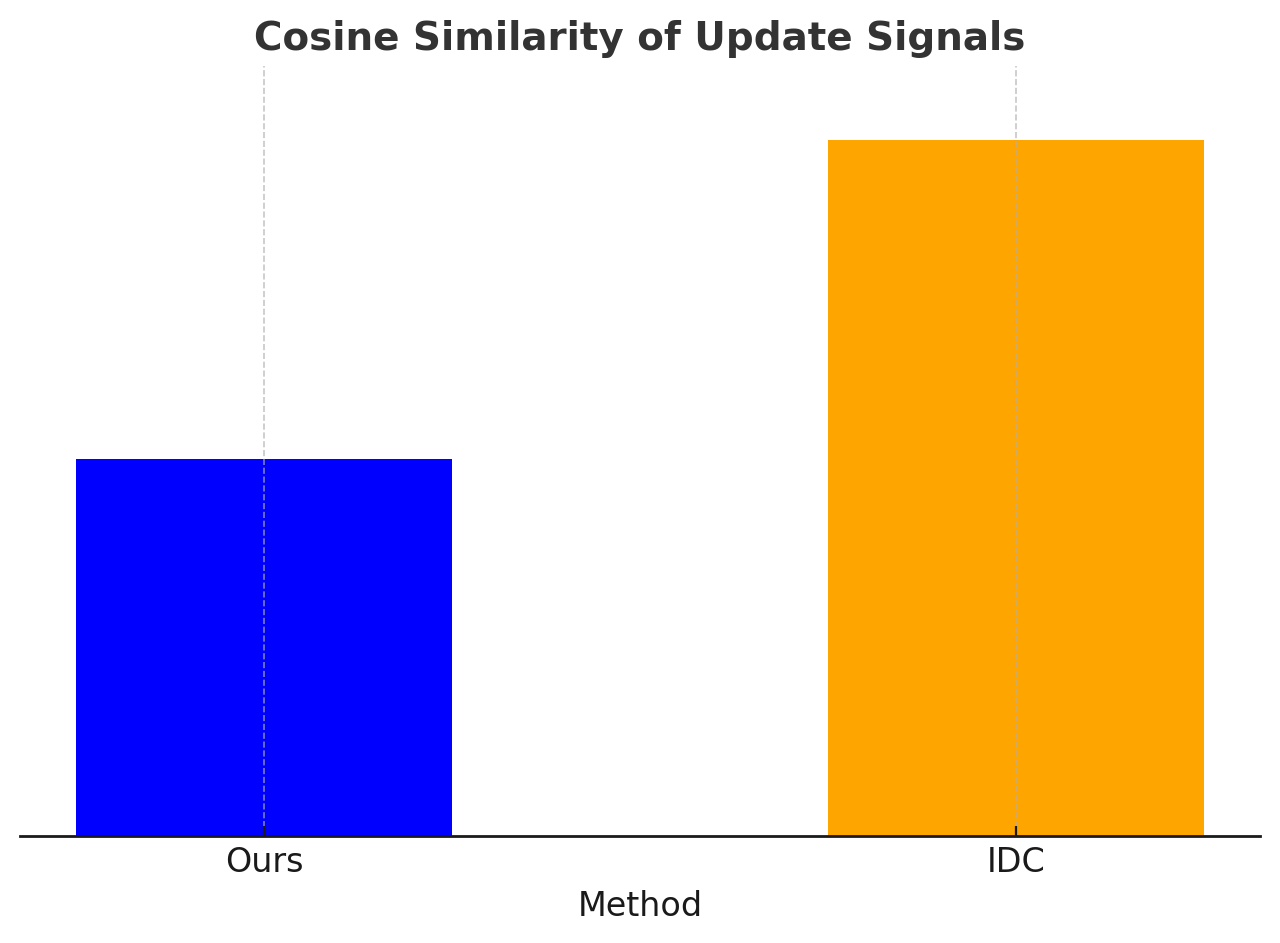
\includegraphics[width=0.5\textwidth]{./images/loss_cosine.png}
    \caption{Cosine similarity of update signals of OUR and IDC method. Update signals are obtained by subtracting initialized images from the generated synthetic images, where both OUR and IDC are initialized with the same set of images. The cosine similarity is averaged for all classes.}
    \label{fig:training_signal}
\end{figure}

\begin{figure}[t]
    \centering
    \begin{subfigure}[b]{0.23\textwidth}  % Ensure the width is valid
        \centering
        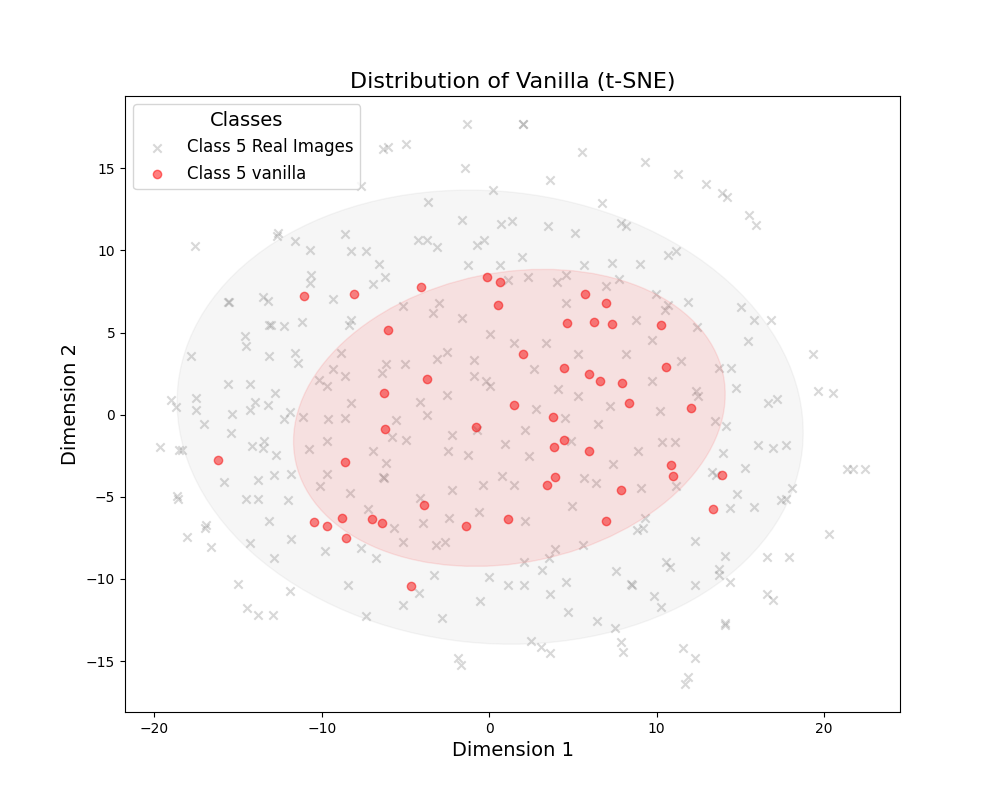
\includegraphics[width=\textwidth]{./images/vanilla.png}  % Verify path and file existence
        \caption{IDC}
        \label{fig:IDC}
    \end{subfigure}
    \hfill
    \begin{subfigure}[b]{0.23\textwidth}  % Ensure the width is valid
        \centering
        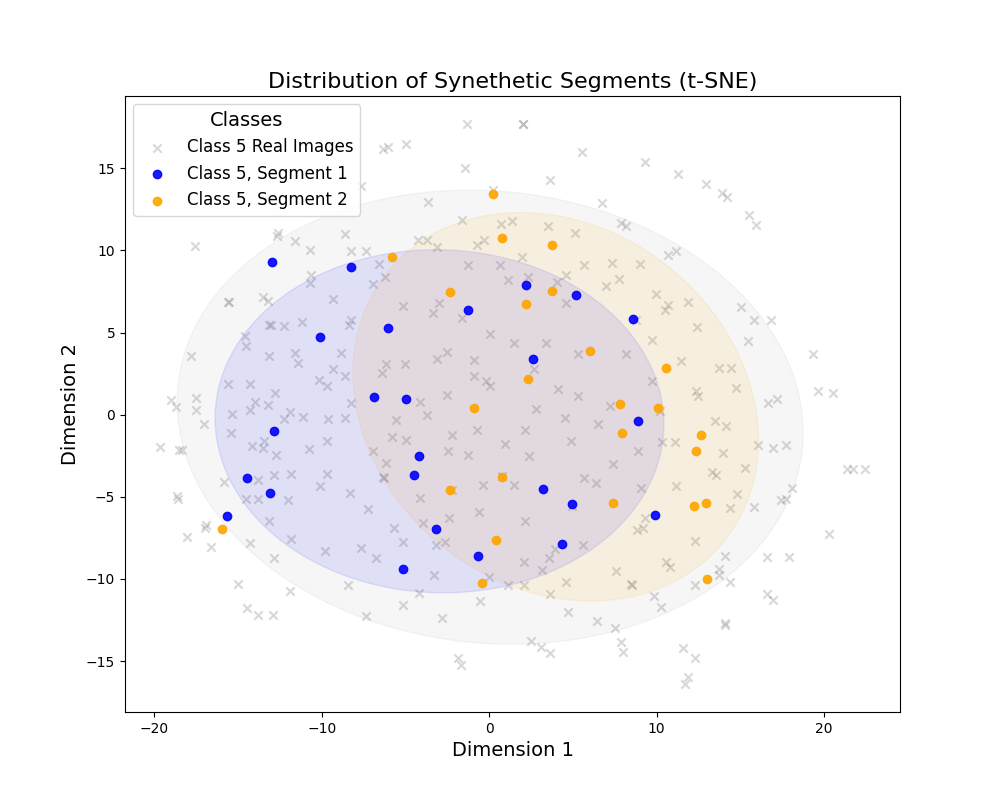
\includegraphics[width=\textwidth]{./images/ours.png}  % Verify path and file existence
        \caption{OURS}
        \label{fig:EDD}
    \end{subfigure}
    
    \caption{T-SNE distribution of synthetic images generated from using our and IDC method. IDC generates synthetic images that are clustered around the center, while our method generates synthetic images that cover a wide distribution. Note that images generated in different segments tend to cover different parts of the distribution.}
    \label{fig:mainfigure}
\end{figure}

Although existing dataset distillation methods~\cite{} demonstrate strong performance when generating synthetic datasets with few images per class (IPC), they fail to scale effectively to higher IPC settings. This limitation arises due to synthetic images being updated simultaneously in a single large batch, where minimizing the features between batches of real and synthetic images causes the individual synthetic images to become similar. The synthetic images are simultaneously updated to minimize the same loss, resulting in similar back-propagation signals across the batch. Consequently, redundant information is embedded in the synthetic images. In contrast, our method divides the synthetic images in to exclusive subsets. Each subset is updated using a different loss. This results in the synthetic images being updated in different directions. This is illustrated in ~Fig.~\ref{fig:training_signal}, where the average cosine similarity of update signals are plotted for IDC~\cite{} and our method. The update signal is obtained by subtracting the initialized image from the generated synthetic image. High cosine similarity of IDC indicates that the synthetic images are being updated in a similar direction, while low cosine similarity of our method shows that synthetic images are updated towards different directions. Furthermore, ~Fig.~\ref{fig:mainfigure} presents T-SNE~\cite{} distribution of synthetic dataset generated by IDC and our method. IDC generates synthetic images that are close in distribution, which indicate the generated synthetic images are similar to each other. On the other hand, our method generates synthetic images that cover a wide range of distribution, demonstrating that it captures diverse aspects of the real dataset.

% \begin{figure}[t]
%     \centering
%     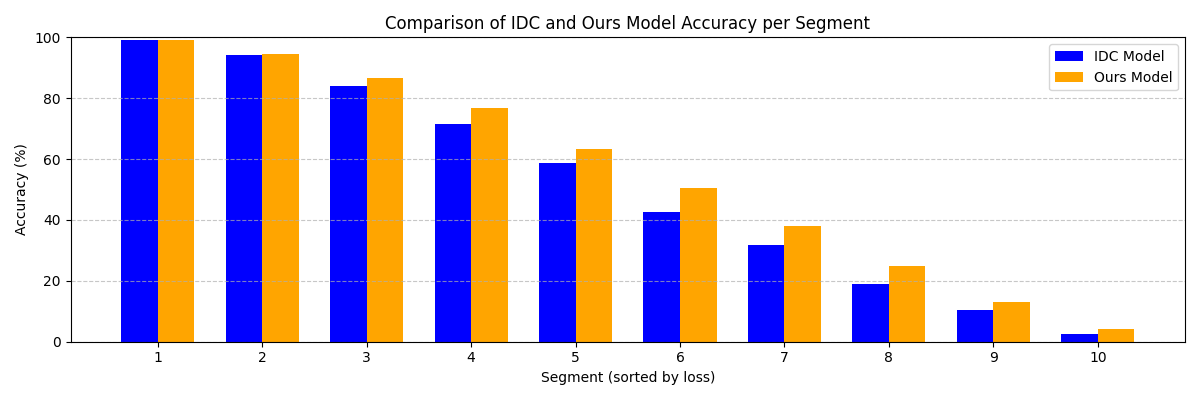
\includegraphics[width=0.5\textwidth]{icml2025/images/loss.png}
%     \caption{Histogram of accuracy for cifar-100 dataset}
%     \label{fig:example_image}
% \end{figure}

In this paper, we propose \textbf{EDD} (Exclusive Dataset Distillation), a novel framework that can be orthogonally integrated into many existing works~\cite{}. To address the issue of shared loss, synthetic images are updated in small exclusive subsets, which we denote as segments. Each segment is then trained by matching different subsets of the real dataset, encouraging the segments to learn different parts of the real dataset. The process begins with generating the first segment. A model is trained with the first segment, which is then used to classify the real dataset, discarding a portion of correctly classified images and retaining mainly the misclassified ones. These misclassified images are used to train the subsequent segment, and the process of generating segments and filtering the real dataset is repeated until the last segment is generated. However, naively training subsequent segments with the filtered dataset results in performance degradation compared to baseline methods. This is mainly due the `forgetting' phenomenon~\cite{} which will be explained in more detail in section 4. To state briefly, adding new segments to existing ones causes the model to misclassify images it previously classified correctly. To address the forgetting phenomenon, we add a regularization loss derived from previously generated segments, used for generating subsequent segments . This regularization loss reduces the forgetting phenomenon, and improves final performance. When integrated into existing approaches, our method demonstrates competitive performance compared to baseline methods, especially for datasets with many classes in high IPC regions. We summarize our contributions as follows:
\begin{itemize}
    \item We propose EDD, a novel framework that allows embedding of exclusive information into synthetic images by training segments with different subsets of the real dataset.
    \item To address the forgetting phenomenon, we add a regularization loss, which reduces the number of forgotten images when adding new segments.
    \item Our method shows competitive performance across a variety of datasets, and especially performs well on datasets with many classes. On the tiny-imagenet 50 ipc setting, our method achieves $44.3\%$ accuracy, surpassing the current SOTA by a $4.6\%$ margin.
\end{itemize}


\section{Related Works}
Dataset distillation compresses real images into synthetic images by optimizing the distance between the features of real and synthetic images. Current research primarily focuses on two strategies: gradient/trajectory matching and distribution matching.

\textbf{Gradient/Trajectory Matching}: The core principle of these methods is that synthetic images should produce back-propagation signals similar to those of real images. DC emphasizes matching one-step gradients, while MTT advances this concept by matching entire training trajectories. Although trajectory matching methods are often regarded as the current SOTA framework for dataset distillation, our experiments reveal that gradient matching methods outperform them on large-scale datasets and high-IPC settings. Furthermore, gradient matching methods demonstrate superior generalization across multiple architectures, which is why we mainly implement our method to gradient matching frameworks.

\textbf{Distribution Matching}: Another approach focuses on aligning the feature maps of real and synthetic data. Early methods such as CAFE and DM adopted this strategy but exhibited inferior performance compared to gradient or trajectory matching frameworks. More recent works propose a novel take on distribution matching, generating synthetic images by aligning the batch normalization statistics of real images. However, these methods are highly memory-intensive, requiring approximately 40 times more memory to store soft labels than is needed for synthetic images. Moreover, synthetic images generated using this approach often perform worse than randomly selected images. Based on these findings, we conclude that this line of work is not well-suited for dataset distillation. Consequently, our focus remains on traditional gradient/trajectory matching methods.



\section{Preliminary}

Dataset distillation is a task of generating a batch of synthetic images $\mathcal{S}$ such that networks trained with $\mathcal{S}$ perform similar to networks that are trained with the original training set $\mathcal{R}$. However, directly optimizing with respect to the generalization performance is very expensive, so surrogate objectives are solved instead to minimize distance between the real and synthetic dataset.

\begin{equation}
R: \text{Real Dataset}
\end{equation}
\begin{equation}
S: \text{Synthetic Dataset}
\end{equation}
\begin{equation}
S^* = \arg \min_{S} \mathcal{D}(S,R)
\end{equation}

The distance between the datasets can be measured in term of feature maps, gradients, or training trajectories. 

The  DASM framework can be implemented into all three surrogate objective methods, but as stated earlier, we work on gradient matching methods due to its superior performance and cross architecture generalization. In particular, we build upon IDC, where gradient matching is performed with downsampled synthetic images.

\begin{equation}
S^* = \arg \min_{S} \mathcal{D} \left( \nabla_{\theta} \mathcal{L}(\theta(\mathcal{A}^*(S))), \nabla_{\theta} \mathcal{L}(\theta(\mathcal{A}(R))) \right)
\end{equation}

$\mathcal{A}$ represents differential siamese augmentation, and $\mathcal{A}^*$ is upsampling followed by $\mathcal{A}$.






% In the unusual situation where you want a paper to appear in the
% references without citing it in the main text, use \nocite
\nocite{langley00}

\bibliography{example_paper}
\bibliographystyle{icml2025}


%%%%%%%%%%%%%%%%%%%%%%%%%%%%%%%%%%%%%%%%%%%%%%%%%%%%%%%%%%%%%%%%%%%%%%%%%%%%%%%
%%%%%%%%%%%%%%%%%%%%%%%%%%%%%%%%%%%%%%%%%%%%%%%%%%%%%%%%%%%%%%%%%%%%%%%%%%%%%%%
% APPENDIX
%%%%%%%%%%%%%%%%%%%%%%%%%%%%%%%%%%%%%%%%%%%%%%%%%%%%%%%%%%%%%%%%%%%%%%%%%%%%%%%
%%%%%%%%%%%%%%%%%%%%%%%%%%%%%%%%%%%%%%%%%%%%%%%%%%%%%%%%%%%%%%%%%%%%%%%%%%%%%%%
\newpage
\appendix
\onecolumn
\section{You \emph{can} have an appendix here.}

You can have as much text here as you want. The main body must be at most $8$ pages long.
For the final version, one more page can be added.
If you want, you can use an appendix like this one.  

The $\mathtt{\backslash onecolumn}$ command above can be kept in place if you prefer a one-column appendix, or can be removed if you prefer a two-column appendix.  Apart from this possible change, the style (font size, spacing, margins, page numbering, etc.) should be kept the same as the main body.
%%%%%%%%%%%%%%%%%%%%%%%%%%%%%%%%%%%%%%%%%%%%%%%%%%%%%%%%%%%%%%%%%%%%%%%%%%%%%%%
%%%%%%%%%%%%%%%%%%%%%%%%%%%%%%%%%%%%%%%%%%%%%%%%%%%%%%%%%%%%%%%%%%%%%%%%%%%%%%%


\end{document}


% This document was modified from the file originally made available by
% Pat Langley and Andrea Danyluk for ICML-2K. This version was created
% by Iain Murray in 2018, and modified by Alexandre Bouchard in
% 2019 and 2021 and by Csaba Szepesvari, Gang Niu and Sivan Sabato in 2022.
% Modified again in 2023 and 2024 by Sivan Sabato and Jonathan Scarlett.
% Previous contributors include Dan Roy, Lise Getoor and Tobias
% Scheffer, which was slightly modified from the 2010 version by
% Thorsten Joachims & Johannes Fuernkranz, slightly modified from the
% 2009 version by Kiri Wagstaff and Sam Roweis's 2008 version, which is
% slightly modified from Prasad Tadepalli's 2007 version which is a
% lightly changed version of the previous year's version by Andrew
% Moore, which was in turn edited from those of Kristian Kersting and
% Codrina Lauth. Alex Smola contributed to the algorithmic style files.
